\subsection{Arsitektur Sistem}
\label{subsection:system-architecture}

\begin{figure}[ht]
    \centering
    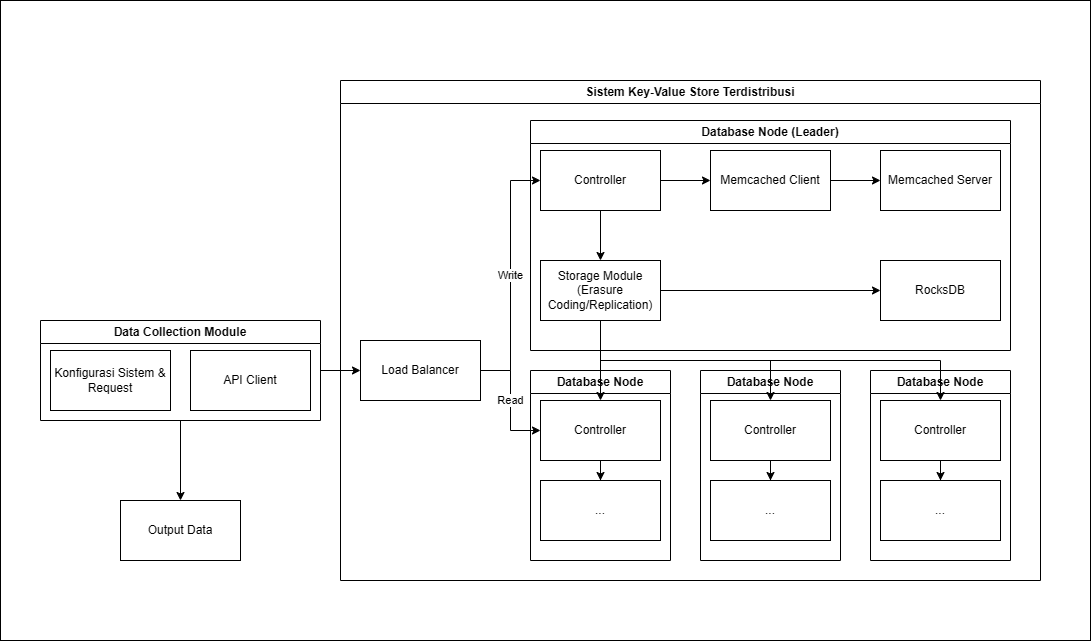
\includegraphics[width=0.95\textwidth]{resources/chapter-3/general-architecture.png}
    \caption{Gambaran Umum Arsitektur Sistem Eksperimen}
    \label{fig:general-architecture}
\end{figure}

Arsitektur dari sistem mengasumsikan kebutuhan untuk konsistensi yang tinggi. Untuk mencapai konsistensi tersebut, operasi \textit{write} dilakukan secara \textit{synchronous} dengan distribusi replikasi dan \textit{erasure coding} dianggap selesai ketika nilai ketahanan yang diinginkan sudah tercapai. Sistem terdistribusi akan mengadopsi pola \textit{leader-follower} untuk memudahkan sinkronisasi data. Pemilihan \textit{leader} dan pemastian transaksi akan dilakukan menggunakan algoritma konsensus \textit{paxos} yang disesuaikan dengan kebutuhan. Diagram gambaran umum arsitektur sistem dapat dilihat pada gambar \ref{fig:general-architecture}.

Operasi akan disalurkan melalui sebuah \textit{load-balancer} sebelum mencapai \textit{database node}. Operasi \textit{write} akan secara ekslusif disalurkan pada \textit{leader}. Kemudian untuk ketahanan, data akan didistribusikan pada \textit{follower} sesuai dengan konfigurasi modul \textit{redundancy}. Sementara itu, operasi \textit{read} dapat dilakukan pada \textit{database node} manapun. Pada sistem \textit{erasure coding}, jika pada \textit{node} tersebut tidak terdapat nilai data yang dicari, maka \textit{node} akan melakukan \textit{request} ke semua node lainnya untuk melakukan rekonstruksi data.

\subsection{Alur Transaksi}
\label{subsection:system-flow}

Alur untuk transaksi \textit{read} dapat dilihat pada gambar \ref{fig:flow-read-mermaidjs} dengan \textit{request} masuk ke \textit{load balancer} kemudian disalurkan ke \textit{database node} yang tersedia. \textit{Database node} akan melakukan operasi \textit{read} pada \textit{key-value store} dan mengembalikan hasil operasi ke \textit{load balancer} untuk dikirimkan ke \textit{client} jika tersedia. Jika tidak, maka \textit{database node} akan melakukan rekonstruksi data dari \textit{erasure-coded persistent data} yang tersebar pada \textit{node-node} lainnya. Pada replikasi, data akan diambil dari \textit{node} lain yang memiliki data yang sama.

\begin{figure}[!ht]
    \centering
    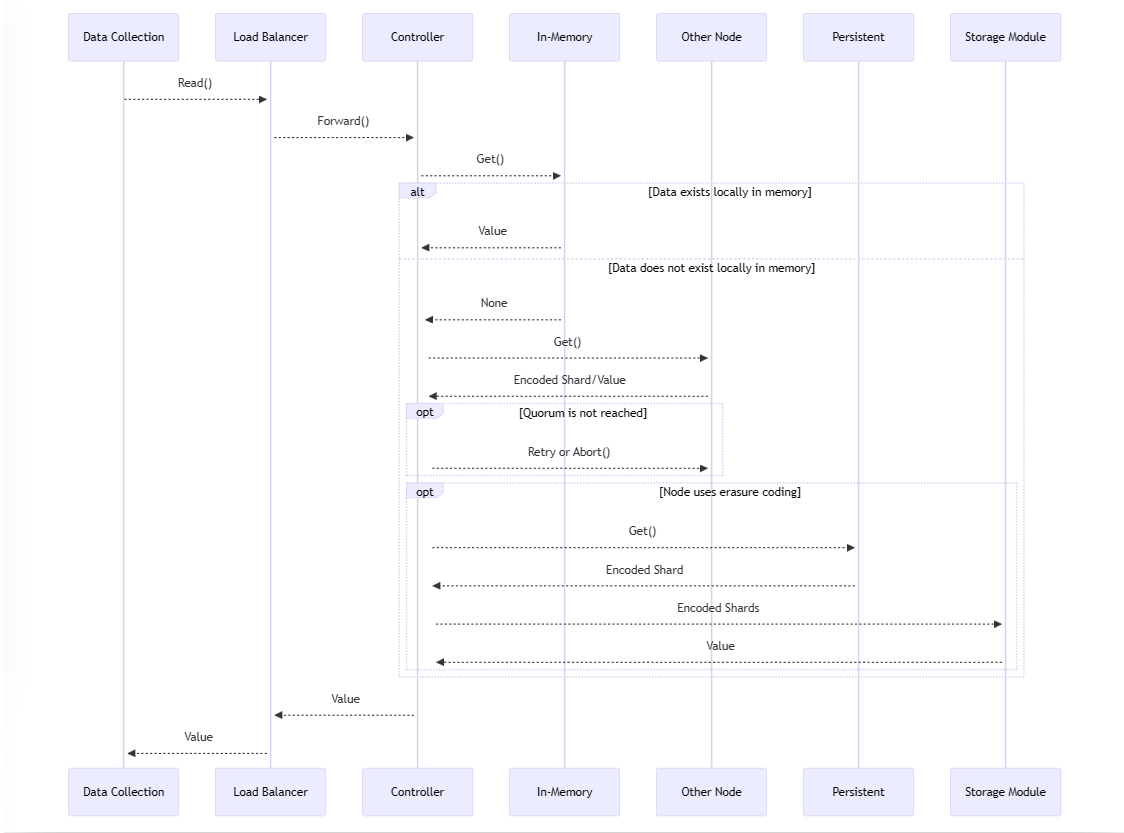
\includegraphics[width=0.95\textwidth]{resources/chapter-3/flow-read-mermaidjs.png}
    \caption{Flow operasi \textit{read} dalam rancangan implementasi}
    \label{fig:flow-read-mermaidjs}
\end{figure}

Alur untuk transaksi \textit{read} dapat dilihat pada gambar \ref{fig:flow-write-mermaidjs} dengan \textit{request} masuk ke \textit{load balancer} kemudian disalurkan ke \textit{database node} yang merupakan leader. Leader kemudian akan melakukan operasi \textit{erasure coding} lalu menyebarkan \textit{shard} ke \textit{follower} yang tersedia. Setelah semua \textit{follower} menerima \textit{shard}, maka operasi \textit{write} dianggap selesai. Operasi \textit{write} pada replikasi juga akan menunggu semua \textit{follower} menerima data sebelum dianggap selesai. 

\begin{figure}[!ht]
    \centering
    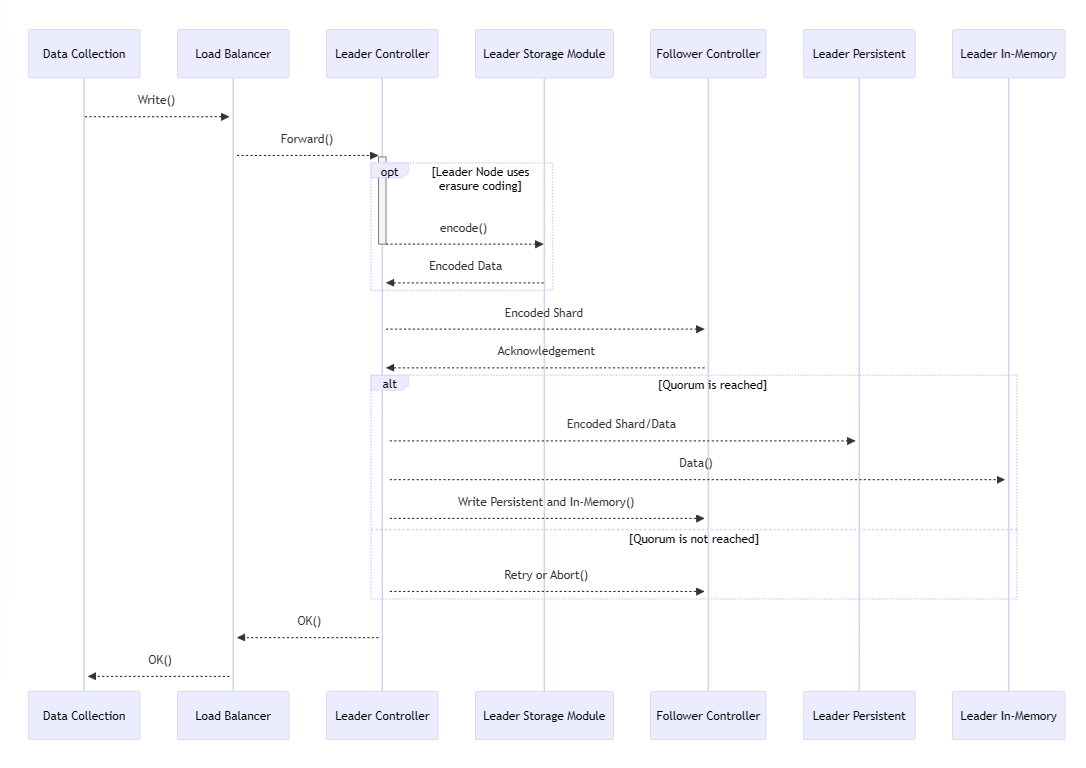
\includegraphics[width=0.95\textwidth]{resources/chapter-3/flow-write-mermaidjs.png}
    \caption{Flow operasi \textit{write} dalam rancangan implementasi}
    \label{fig:flow-write-mermaidjs}
\end{figure}
